\section{Additional Experiments}
\label{app:add}

\begin{figure}[t]
\centering
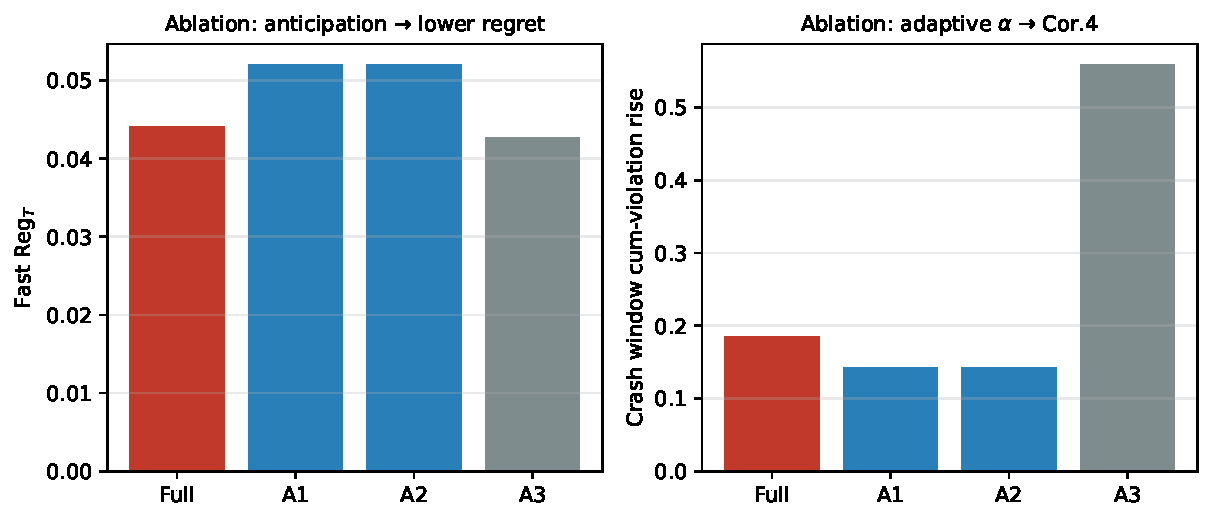
\includegraphics[width=0.9\linewidth]{figures/figE_ablation.pdf}
\caption{Ablation summary: Fast-regime regret (left) and crash-window cumulative-violation rise (right).
Demonstrates the empirical behavior predicted by Corollary~\ref{cor:4} (adaptive $\alpha$ vs.\ $\alpha\equiv 1$).}
\label{fig:ablation}
\end{figure}

Fig.~\ref{fig:ablation} expands Table~\ref{tab:ablation}.
A1/A2 coincide operationally when $\alpha=0$ (projection onto $\mathcal{B}(c_t)$).
A3 ($\alpha\equiv 1$) nearly matches Full on clean Fast UAV but inflates crash-window rise by $\approx 3\times$, isolating failure containment.

\paragraph{Evidence chain.}
Claims map to theory and figures as: Thm.~\ref{thm:1}~$\leftrightarrow\delta$ logs;
Lem.~\ref{lem:2}~$\leftrightarrow$ Oracle gap;
Thm.~\ref{thm:2}~$\leftrightarrow$ Fig.~\ref{fig:regret} \& Table~\ref{tab:drift};
Thm.~\ref{thm:3}~$\leftrightarrow$ Fig.~\ref{fig:pi};
Cor.~\ref{cor:4}~$\leftrightarrow$ Fig.~\ref{fig:crash} \& A3.
